% EDIT HERE: complete supplementary material, including all tables and figures.
% References: main.bib.
\documentclass[10pt,onecolumn,letterpaper]{article}
\usepackage[review]{cvpr}
% ===== BEGIN preamble =====
% Explicit dependencies used by the manuscript (not reviewer-facing definitions).
\usepackage{graphicx}
\usepackage{amsmath}
\usepackage{amssymb}
\usepackage{booktabs}
\usepackage{microtype}
\usepackage{placeins}
\usepackage{colortbl}
\definecolor{oursbg}{RGB}{255,247,225}
\definecolor{resultgold}{RGB}{153,117,16}
\definecolor{resultgray}{RGB}{95,102,110}
\newcommand{\na}{\textcolor{black!40}{n/a}}
\newcommand{\nev}{\textcolor{black!40}{--}}
\usepackage{xspace}
\newcommand{\ours}{REVAMAP\xspace}
\newcommand{\tgroup}[2]{\multicolumn{#1}{@{}l}{\textit{#2}}\\}

% Table shading represents rank, independently of method identity.
\definecolor{rankbest}{RGB}{205,225,250}
\definecolor{ranksecond}{RGB}{240,246,253}
\newcommand{\rankbestcell}[1]{\begingroup\setlength{\fboxsep}{1.5pt}\colorbox{rankbest}{\kern1.2pt\textbf{#1}\kern1.2pt}\endgroup}
\newcommand{\ranksecondcell}[1]{\begingroup\setlength{\fboxsep}{1.5pt}\colorbox{ranksecond}{\kern1.2pt#1\kern1.2pt}\endgroup}
\newcommand{\ranklegend}{\begingroup\setlength{\fboxsep}{0.7pt}\colorbox{rankbest}{best}/\colorbox{ranksecond}{second}\endgroup}
% ===== END preamble =====
\usepackage{xcolor}
\usepackage{multirow}
\definecolor{cvprblue}{rgb}{0.21,0.49,0.74}
\usepackage[pagebackref,breaklinks,colorlinks,allcolors=cvprblue]{hyperref}
\def\confName{CVPR}
\def\confYear{2027}
\title{REVAMAP: Reconstruction from Evolving Views Across Maps and Passes\\Supplementary Material}
\author{Anonymous Authors}
\begin{document}
\maketitle
\vspace{-9mm}
\renewcommand{\thetable}{S\arabic{table}}
\renewcommand{\thefigure}{S\arabic{figure}}
% ===== BEGIN sec / method_details =====
\renewcommand{\thesection}{\Alph{section}}
\section{Method Details}
\label{sec:supp_method}

Every dense map fuses observations into its elements: TSDF volumes average them, Gaussian maps take gradient steps on a
rendering loss, and occupancy maps sum log-odds. \ours keeps each native rule and only decides which observations may
enter it. An observation $o$ captured at $t_o$ is valid for an element $e$ at time $t$ if $e$ existed then and exists
now (Eq.~3 of the main paper),
\begin{equation}
  v_o(e,t)=\bigl[\,e\in\mathcal{M}(t_o)\cap\mathcal{M}(t)\,\bigr]\in\{0,1\},
  \label{eq:supp_valid}
\end{equation}
and each map applies $v$ inside its own update:
\begin{align}
  D_t(x)&=\frac{\sum_o v_o(x,t)\,w_o(x)\,d_o(x)}{\sum_o v_o(x,t)\,w_o(x)},
  \qquad v_o(x,t)=\bigl[\sigma_o\in\mathcal{S}(t)\bigr]\,\bigl[x\in\Omega_o(t)\bigr],\label{eq:supp_tsdf}\\
  \theta_e&\leftarrow\theta_e-\alpha\sum_k v_k(e,t)\,\frac{\partial\,\ell\bigl(I_k,R(\mathcal{M}(t_k))\bigr)}{\partial\theta_e},\label{eq:supp_gs}\\
  L(c)&\leftarrow\mathrm{clamp}\bigl(L(c)+v_o(c,t)\,\Delta_o(c)\bigr).\label{eq:supp_occ}
\end{align}
In \cref{eq:supp_tsdf}, the signed distance $D$ of a voxel $x$ is the weighted mean of the ray distances $d_o$. A pixel
ray $o$ ends on a state $\sigma_o$ or on the background, $\mathcal{S}(t)$ is the set of states alive at $t$, and
$\Omega_o(t)$ is the valid domain (Eq.~4 of the main paper). A ray counts only while the state it hit still stands; its
band keeps the surface it measured, and its free space stops before the first state that arrived after $t_o$. The wall
thus keeps its old views, the departed armchair loses its own, and views taken before the sofa arrived never carve it.
A state that starts or ends re-fuses only the voxel blocks its rays cross, from archived frames.
In \cref{eq:supp_gs}, keyframe $k$ with image $I_k$ renders the map of its capture time, $R(\mathcal{M}(t_k))$, and its
gradient reaches only the Gaussians alive both then and now; ended Gaussians stay frozen.
In \cref{eq:supp_occ}, a cell $c$ keeps only the clamped sum of its updates $\Delta_o$, not which observation
contributed what, so $v$ is applied at the two ends of a state, the only times it changes. At its start, the first
object reading of a visit in a cell that earlier visits saw free withdraws the value $L_0(c)<0$ that the cell held when
the visit began, $L(c)\leftarrow L(c)-L_0(c)$, so the cell keeps only the evidence of the current visit. At its end,
the cells of the state are set to the free bound $L_{\min}$. The state intervals that
define $\mathcal{M}$ and $\mathcal{S}$ come from change detection.

\paragraph{Change detection.}
Each depth image tests at most 1,500 surface samples per state, with a depth tolerance equal to the map resolution
(a 5\,cm reference scale for Gaussians) and an incidence limit of $60^\circ$. A round needs at least
$\min(30,\nu_{\mathrm{rel}})$ judged samples, where $\nu_{\mathrm{rel}}$ is the number of reliable samples of the state,
and $f_i=k_i/n_i$ is the fraction of the $n_i$ inspected samples that round $i$ sees through. A round is in place when
more of its samples carry the state's own mask than are seen through, and it is scored before it can join the in-place
statistics, so rounds after a change never enter the model. The Beta moments are fitted per object from its third
in-place round on and shrunk toward the pool of all objects, weighted as three rounds; the variance never falls below
the spread between objects or $10^{-4}$, and the concentration is at least two. Without a pool, the model is
$\mathrm{Beta}(0.1,1.9)$, a 5\% see-through rate, and fractions are clamped between the fitted mean and 0.995 before
computing the one-sided log-density ratio $\ell_s(f_i)$. The weight $w_i(j)=\nu_i(j)/\nu_{\mathrm{rel}}$ divides the
number $\nu_i(j)$ of reliable samples inspected for the first time since the candidate change time $j$ by
$\nu_{\mathrm{rel}}$, so each sample contributes once per candidate window. We use $\eta=99$ in all experiments.
Persistence is estimated from unchanged and moved outcomes using a Beta prior from the object's class, with the class
estimate smoothed toward its mobility group. A state begins when it is first seen and ends at its confirming round,
which bounds the unobserved departure from above. For a removed object, the exported TSDF map places the end midway
between the last supporting observation and the confirming round, as Khronos~\cite{Schmid-RSS-24} does, and a Gaussian
state that changed between visits ends at the start of the current visit.

\section{Datasets}
\label{sec:supp_datasets}

ReviScene-BedRoom (\cref{fig:supp_bedroom}) has 4,003, 4,041, and 7,216 RGB-D frames in its three visits, at
1920$\times$1080 and 30\,Hz, with depth aligned to RGB. We register visits B and C to A using landmark correspondences,
automatic registration, and manual refinement. Masks combine SAM assistance and manual review, with ADE20K classes and
17 persistent object IDs; people are labeled dynamic. No ethics review was carried out because the only person recorded
is a volunteer who consented to the recording; faces are blurred. ReviScene-Home (\cref{fig:supp_home}) animates objects
and camera trajectories in the kujiale\_0021 apartment of InteriorAgent~\cite{InteriorAgent2025}. Its two visits share a
world coordinate frame and have 4,186 and 3,555 RGB-D frames at 680$\times$480 and 30\,Hz. We export per-frame object
transforms and visibility, which give the scene geometry at each timestamp together with the object meshes. Instance
labels follow the annotated object groups, such as a table together with its contents. Among the public datasets, Flat
moves eight objects, adds five, and removes four between its two runs~\cite{9811877}, and we use eight room chains of
3RScan~\cite{9010673}.

\begin{figure}[!htb]
\centering
\newcommand{\bedpanel}[2]{\begin{minipage}[t]{0.243\linewidth}\centering{\footnotesize #1}\par\vspace{1pt}%
\includegraphics[width=\linewidth,trim=170bp 150bp 170bp 0bp,clip]{figures/real_stages_original/#2.png}\end{minipage}}
\bedpanel{Visit A, 85.0\,s}{a_before}\hfill\bedpanel{Visit A, 133.3\,s}{a_after}\hfill\bedpanel{Visit B, 34.0\,s}{b_before}\hfill\bedpanel{Visit B, 134.5\,s}{b_after}\\[4pt]
\bedpanel{Visit C, 30.0\,s}{c_before}\hfill\bedpanel{Visit C, 100.0\,s}{c_middle}\hfill\bedpanel{Visit C, 240.0\,s}{c_after}\hfill\begin{minipage}[t]{0.243\linewidth}\mbox{}\end{minipage}
\caption{\textbf{ReviScene-BedRoom from a fixed overview camera.} The luggage appears beside the wall during visit A, moves toward the bed during visit B, and during visit C moves from beside the desk to the clothes rack and then toward the bed. The room is also rearranged between visits.}
\label{fig:supp_bedroom}
\end{figure}

\begin{figure}[!htb]
\centering
\newcommand{\homepanel}[2]{\begin{minipage}[t]{0.243\linewidth}\centering{\footnotesize #1}\par\vspace{1pt}%
\includegraphics[width=\linewidth]{figures/dataset_stages/#2_rgb.png}\end{minipage}}
\homepanel{Visit A, 0\,s: initial layout}{a_0000.00}\hfill\homepanel{Visit A, 80\,s: after cabinet motion}{a_0080.00}\hfill\homepanel{Visit A, 95\,s: furniture rearranged}{a_0095.00}\hfill\homepanel{Visit A, 125\,s: side table moved}{a_0125.00}\\[4pt]
\homepanel{Visit A, 139.5\,s: chair moved}{a_0139.50}\hfill\homepanel{Visit B, 0\,s: initial layout}{b_0000.00}\hfill\homepanel{Visit B, 35\,s: side table moved}{b_0035.00}\hfill\homepanel{Visit B, 50\,s: chair moved}{b_0050.00}\\[4pt]
\homepanel{Visit B, 65\,s: furniture rearranged}{b_0065.00}\hfill\homepanel{Visit B, 90\,s: cabinet moved}{b_0090.00}\hfill\homepanel{Visit B, 118.4\,s: plant moved}{b_0118.40}\hfill\begin{minipage}[t]{0.243\linewidth}\mbox{}\end{minipage}
\caption{\textbf{ReviScene-Home from a fixed overview camera.} Isaac Sim renders of the successive arrangements in the two visits. The start of visit B shows the bedroom and living room rearranged between the visits.}
\label{fig:supp_home}
\end{figure}

\section{Evaluation Details}

Each method continues through the chain of visits using its own map updates. Panoptic Mapping loads the preceding
visit's map through its native interface and uses 5\,cm object and background resolution. The GaME 3RScan run uses its
dataset-adapted implementation. On real RGB-D, invalid depths are excluded from geometry supervision and allocation;
the synthetic GaME adapter corrects relative-pose keyframe selection and guards sampling termination. Flat uses the
original GaME configuration. For 3RScan, evaluation images are 480$\times$270 for both Gaussian methods; in three
rooms, Gaussian mapping uses 240$\times$135 inputs to fit memory.

Following Khronos~\cite{Schmid-RSS-24}, object matching uses a 0.5\,m distance threshold, and scores at successive
snapshots are weighted by the duration for which each snapshot is current. For 3RScan, scores are first averaged over
visits within a room and then over eight rooms. Change F1 pools true positives, false positives, and false negatives
across the complete chain; 3RScan contains 77 pooled reference events. The state-based 3RScan evaluator considers a
reference state represented when at least half its points lie within 10\,cm of a single mapped object surface. An
earlier state that is no longer represented supplies disappearance evidence; a new represented state supplies
appearance evidence. A persistent reference object reported as disappeared is a false positive. Gaussian and occupancy
exports form object components using 26-connectivity on a 10\,cm grid within each identity, accepting components of
volume 0.005--10\,m$^3$, following the Khronos object construction settings; the same rule is used for a
representation's native and proposed updates. Panoptic snapshots are recorded every 2\,s of dataset time; Absent
submaps supply disappearance decisions, while Unobserved submaps do not.

\section{Additional Results}

\paragraph{Changes by kind.}
\Cref{tab:supp_change_kinds} splits the change F1 of the main paper into changes after looking away within a visit and
changes across visits.

\begin{table}[!htb]
\centering
\fontsize{9}{10.3}\selectfont
\setlength{\tabcolsep}{3.2pt}
\renewcommand{\arraystretch}{1.08}
\begin{tabular}{@{}ll*{4}{r}@{}}
\toprule
& & \multicolumn{2}{c}{BedRoom} & \multicolumn{2}{c}{Home} \\ \cmidrule(lr){3-4}\cmidrule(lr){5-6}
Map & Method & Away & Across & Away & Across \\ \midrule
TSDF & Khronos & 57.1 & 73.2 & 81.7 & 86.7 \\
 & Panoptic & 36.4 & 54.1 & 76.9 & 69.2 \\
 & Ours & 100.0 & 98.0 & 100.0 & 95.4 \\
\midrule
3DGS & GaME & 100.0 & 96.0 & 83.1 & 82.8 \\
 & Ours & 100.0 & 98.0 & 100.0 & 95.4 \\
\midrule
Occupancy & Wavemap & 90.9 & 89.4 & 98.7 & 93.8 \\
 & Ours & 100.0 & 100.0 & 100.0 & 97.0 \\
\bottomrule
\end{tabular}
\caption{\textbf{Change F1 by kind of change.} F1 (\%) for changes after looking away within a visit (\emph{Away}) and across visits. The change F1 of the main paper pools the two. BedRoom has 5 and 26 such events; Home has 38 and 34.}
\label{tab:supp_change_kinds}
\end{table}

\paragraph{Geometry at each visit.}
\Cref{tab:supp_geometry} reports mesh F1 at the end of every visit; the final-visit Gaussian scores use the refined
maps. The synthetic reference here consists of the ground-truth surfaces observed up to the evaluation time, whereas
the Home columns of the main paper use the complete ground-truth mesh of the apartment. \Cref{tab:supp_restart}
compares native maps rebuilt from scratch with our continued maps.

\begin{table}[!htb]
\centering
\fontsize{9}{10.3}\selectfont
\setlength{\tabcolsep}{5pt}
\renewcommand{\arraystretch}{1.08}
\begin{tabular}{@{}l*{8}{r}@{}}
\toprule
F1$\uparrow$ & \multicolumn{3}{c}{BedRoom} & \multicolumn{2}{c}{Home} & \multicolumn{2}{c}{Flat} & 3RScan \\
\cmidrule(lr){2-4}\cmidrule(lr){5-6}\cmidrule(lr){7-8}
Method & A & B & C & A & B & A & B & Mean \\ \midrule
Khronos & 90.9 & 88.9 & 87.7 & 93.6 & 93.1 & 86.0 & 86.9 & 88.8 \\
Panoptic & 82.6 & 86.2 & 87.3 & 89.2 & 92.4 & 85.1 & 89.4 & 81.0 \\
Ours (TSDF) & 94.6 & 96.2 & 96.1 & 99.2 & 99.2 & 86.5 & 90.1 & 91.8 \\
\midrule
GaME & 93.2 & 88.6 & 88.6 & 94.9 & 91.3 & 86.6 & 86.2 & 85.9 \\
Ours (3DGS) & 93.5 & 93.1 & 95.1 & 97.7 & 96.5 & 86.3 & 89.8 & 89.6 \\
\midrule
Wavemap & 87.2 & 81.2 & 84.5 & 92.2 & 93.2 & 79.5 & 80.2 & 75.6 \\
Ours (Occ.) & 87.9 & 89.1 & 91.0 & 92.4 & 94.2 & 79.5 & 82.4 & 79.4 \\
\bottomrule
\end{tabular}
\caption{\textbf{Mesh F1 at each visit.} F1 (\%) at 5\,cm; 3RScan uses the room-wise averaging described in the text.}
\label{tab:supp_geometry}
\end{table}

\begin{table}[!htb]
\centering
\fontsize{9}{10.3}\selectfont
\setlength{\tabcolsep}{5pt}
\renewcommand{\arraystretch}{1.08}
\begin{tabular}{@{}lll*{6}{r}@{}}
\toprule
& & & \multicolumn{3}{c}{Native restart} & \multicolumn{3}{c}{Ours, continued} \\ \cmidrule(lr){4-6}\cmidrule(lr){7-9}
Dataset & Map & Visit & P$\uparrow$ & R$\uparrow$ & F1$\uparrow$ & P$\uparrow$ & R$\uparrow$ & F1$\uparrow$ \\ \midrule
BedRoom & TSDF & A & 85.62 & 96.87 & 90.90 & 93.22 & 95.94 & 94.56 \\
 & TSDF & B & 93.71 & 98.28 & 95.94 & 94.93 & 97.47 & 96.18 \\
 & TSDF & C & 91.33 & 98.62 & 94.83 & 93.62 & 98.81 & 96.14 \\
 & 3DGS & A & 95.53 & 91.00 & 93.21 & 95.98 & 91.19 & 93.52 \\
 & 3DGS & B & 95.86 & 91.47 & 93.62 & 92.15 & 94.00 & 93.07 \\
 & 3DGS & C & 97.00 & 93.72 & 95.33 & 95.36 & 94.68 & 95.01 \\
 & Occupancy & A & 81.69 & 93.43 & 87.17 & 81.72 & 95.02 & 87.87 \\
 & Occupancy & B & 86.79 & 90.84 & 88.77 & 85.44 & 93.10 & 89.11 \\
 & Occupancy & C & 82.41 & 96.66 & 88.97 & 84.72 & 98.36 & 91.03 \\
\midrule
Home & TSDF & A & 98.38 & 89.33 & 93.64 & 99.74 & 98.63 & 99.18 \\
 & TSDF & B & 98.10 & 77.57 & 86.63 & 99.80 & 98.66 & 99.23 \\
 & 3DGS & A & 94.02 & 95.85 & 94.92 & 97.01 & 98.49 & 97.74 \\
 & 3DGS & B & 93.30 & 78.72 & 85.39 & 97.15 & 95.99 & 96.57 \\
 & Occupancy & A & 93.00 & 91.48 & 92.24 & 93.13 & 91.68 & 92.40 \\
 & Occupancy & B & 96.49 & 76.50 & 85.34 & 94.90 & 93.58 & 94.23 \\
\bottomrule
\end{tabular}
\caption{\textbf{Restart versus continued mapping.} Precision, recall, and F1 at 5\,cm (\%). Native restart maps and our continued maps are compared after online mapping using the same visit-specific reference.}
\label{tab:supp_restart}
\end{table}

\paragraph{Single visits.}
\Cref{tab:supp_single} evaluates each real and synthetic visit from an empty map with the official evaluator of
Khronos, as on TESSE. The reference state sequence is restricted to that visit: objects present at its start are
initially present, and changes between visits are excluded from its event set. Dynamic references are people in the
real sequences and objects moved in front of the camera in the synthetic sequences. The official evaluator omits
queries with zero true positives from the F1 average. We use a 5\,cm background matching tolerance, and our background
export includes current and historical object geometry, as the Khronos background mesh does. The mesh F1 column
compares the last map with that visit's surface reference and therefore differs from the historical background score.

\begin{table}[!htb]
\centering
\fontsize{9}{10.3}\selectfont
\setlength{\tabcolsep}{2.3pt}
\renewcommand{\arraystretch}{1.08}
\begin{tabular}{@{}ll*{5}{r}@{}}
\toprule
& & Background & Static objects & Dynamic objects & Changes & Mesh \\
Scene & Method & F1$\uparrow$ & F1$\uparrow$ & F1$\uparrow$ & F1$\uparrow$ & F1$\uparrow$ \\ \midrule
BedRoom A & Khronos & 80.6 & 94.3 & -- & 54.2 & 90.9 \\
 & Ours & 84.6 & 96.4 & 96.0 & 97.0 & 94.6 \\
\midrule
BedRoom B & Khronos & 86.6 & 92.4 & 28.2 & 42.0 & 95.9 \\
 & Ours & 87.7 & 95.9 & 88.4 & 66.7 & 97.4 \\
\midrule
BedRoom C & Khronos & 86.7 & 84.1 & 3.3 & 46.0 & 94.8 \\
 & Ours & 88.9 & 93.3 & 97.0 & 85.7 & 97.0 \\
\midrule
Home A & Khronos & 77.0 & 69.5 & 2.8 & 63.5 & 93.6 \\
 & Ours & 92.1 & 77.0 & 73.6 & 71.3 & 99.2 \\
\midrule
Home B & Khronos & 63.8 & 68.5 & 62.6 & 43.7 & 86.6 \\
 & Ours & 77.1 & 77.9 & 73.9 & 59.2 & 89.9 \\
\bottomrule
\end{tabular}
\caption{\textbf{Independent single-visit runs.} F1 scores (\%) follow Khronos's official query aggregation. Final meshes are evaluated using the F1 score at 5\,cm.}
\label{tab:supp_single}
\end{table}

\paragraph{Rendering.}
\Cref{tab:supp_instance_rendering} reports the rendering quality of the Gaussian runs of the main comparison, which
use instance masks. Every tenth frame of the final visit is held out, except the first. LPIPS uses the AlexNet
backbone, and depth L1 is evaluated on pixels with valid measured depth in both methods. The 3RScan result is the mean
over the final visit of each of eight rooms.

\begin{table}[!htb]
\centering
\small
\setlength{\tabcolsep}{3pt}
\begin{tabular}{@{}llrrrr@{}}
\toprule
Scene & Method & PSNR$\uparrow$ & MS-SSIM$\uparrow$ & LPIPS$\downarrow$ & L1$\downarrow$\\
\midrule
BedRoom & GaME & 18.22 & 0.758 & 0.454 & 6.03\\
 & Ours & 19.90 & 0.811 & 0.370 & 4.96\\
Home & GaME & 21.85 & 0.757 & 0.313 & 23.94\\
 & Ours & 24.90 & 0.824 & 0.215 & 15.32\\
Flat & GaME & 24.21 & 0.917 & 0.164 & 1.07\\
 & Ours & 28.43 & 0.955 & 0.107 & 0.41\\
3RScan & GaME & 20.10 & 0.739 & 0.401 & 4.95\\
 & Ours & 21.06 & 0.774 & 0.366 & 2.79\\
\bottomrule
\end{tabular}
\caption{\textbf{Gaussian rendering on the main-comparison sequences.} Held-out views after refinement;
PSNR in dB and depth L1 in cm.}
\label{tab:supp_instance_rendering}
\end{table}

\paragraph{Historical rendering.}
After both visits of Home, we query historical maps at 24 times $T$ and render from the poses of keyframes captured by
$T$. The reference depicts the scene at $T$: we use the original image when the scene has not changed since capture,
and otherwise render it in Isaac Sim at $T$ from the same pose. Both methods use identical views and references before
refinement; GaME uses saved snapshots (\cref{tab:supp_historical_rendering}).

\begin{table}[!htb]
\centering
\small
\begin{tabular}{lr}
\toprule
Method & PSNR$\uparrow$ \\
\midrule
GaME snapshots & 22.99 \\
\rowcolor{oursbg}
\textbf{Ours (history queries)} & \textbf{24.01} \\
\bottomrule
\end{tabular}
\caption{\textbf{Historical rendering on Home before refinement.} PSNR (dB), averaged over views within each time and then across 24 times.}
\label{tab:supp_historical_rendering}
\end{table}

\paragraph{Held-out views of both visits.}
The protocol of GaME~\cite{Yugay_2026_CVPR} holds out frames of the last visit only. For this experiment on Home, we
apply the same rule to the first visit as well (418 and 355 held-out frames), and run both methods again without these
frames. \Cref{tab:supp_heldout_history} reports two queries. The first uses the map of the mapping round that contains
the frame, and is the one reported in the main paper. The second uses the last map before the frame; it is up to
10.8\,s old, so regions the camera has just entered are often missing, for both methods alike. All maps are rendered
before refinement, since refining the map of every time would take about 30 minutes each. The values exceed those on
Home in \cref{tab:supp_instance_rendering}, where every held-out frame is rendered from the final map: Home changes
within its visits, so the final map no longer shows what a frame saw before a later change.

\begin{table}[!htb]
\centering
\small
\setlength{\tabcolsep}{3.2pt}
\begin{tabular}{@{}llrrrrrr@{}}
\toprule
& & \multicolumn{2}{c}{PSNR$\uparrow$} & \multicolumn{2}{c}{MS-SSIM$\uparrow$} & \multicolumn{2}{c}{LPIPS$\downarrow$} \\
\cmidrule(lr){3-4}\cmidrule(lr){5-6}\cmidrule(lr){7-8}
Query & Method & A & B & A & B & A & B \\
\midrule
Round of & GaME & 24.19 & 25.87 & 0.872 & 0.898 & 0.245 & 0.207 \\
the frame & \textbf{Ours} & \textbf{26.64} & \textbf{26.92} & \textbf{0.919} & \textbf{0.926} & \textbf{0.199} & \textbf{0.149} \\
\midrule
Last map & GaME & 15.28 & 18.29 & 0.604 & 0.646 & 0.521 & 0.452 \\
before & \textbf{Ours} & \textbf{16.39} & \textbf{18.87} & \textbf{0.646} & \textbf{0.696} & \textbf{0.483} & \textbf{0.385} \\
\bottomrule
\end{tabular}
\caption{\textbf{Held-out views of both visits on Home, each at its own time.} A: first visit, B: second visit; PSNR in dB. The second query scores 386 frames of A, since the first 32 precede the first map.}
\label{tab:supp_heldout_history}
\end{table}

\paragraph{CL-Splats.}
For reference, we run the public code of CL-Splats~\cite{Ackermann_2025_ICCV} (commit \texttt{587fffc}) on Flat and
Aria with its released default configuration (\cref{tab:supp_clsplats}). The first visit trains the initial scene and
the training frames of the second visit form the update, each with 30{,}000 iterations. CL-Splats receives the same
poses and RGB images, with initial points from the depth of the first visit, and is scored on the same held-out views.
It takes no depth during optimization and is designed for a small set of images of a locally changed region, whereas
each of our visits covers the whole scene. On Aria room1 and Flat, one nearest-neighbour search of the released code is
evaluated in chunks to fit a 16\,GB GPU, which does not change its result.

\begin{table}[!htb]
\centering
\small
\setlength{\tabcolsep}{4pt}
\begin{tabular}{@{}lrrrr@{}}
\toprule
Scene & PSNR$\uparrow$ & MS-SSIM$\uparrow$ & LPIPS$\downarrow$ & L1$\downarrow$\\
\midrule
Flat & 17.91 & 0.677 & 0.397 & 34.8\\
Aria room0 & 21.18 & 0.784 & 0.338 & 32.2\\
Aria room1 & 21.73 & 0.753 & 0.508 & 96.3\\
\bottomrule
\end{tabular}
\caption{\textbf{CL-Splats with its released code and default configuration.} Same held-out views and metrics as Tab.~4 of the main paper; PSNR in dB and depth L1 in cm.}
\label{tab:supp_clsplats}
\end{table}

\section{Further Ablations}

\paragraph{Gaussian maps on Flat.}
\Cref{tab:supp_ablations} extends the ablation table of the main paper. The object and local-surface variants restrict
the application scope of the same change rule, and both recover most of the full result. Without the handover of
states across visits, change F1 drops by one event, to 80.0, and the geometry is unchanged; within the object-scope
variant, removing handover reduces mesh F1 from 89.76 to 84.40 and change F1 from 83.33 to 68.75. \emph{All dynamic
views} samples an earlier keyframe without replay weights, supervises the current map on all pixels, and lets it
optimize currently alive Gaussians. \emph{No dynamic views} drops a keyframe of either visit once it observes a
Gaussian whose lifetime later ends, and a rejected draw is replaced to keep the optimization budget. Both start from
the same saved visit-A map as the full method. Allowing unrestricted reuse only during refinement is as harmful
(22.78\,dB). Rejecting only the first-visit keyframes that observe at least 50 pixels of ended geometry costs 0.65\,dB,
so most of the loss of \emph{No dynamic views} comes from the current-visit keyframes: a second-visit keyframe that
sees the empty floor is the very evidence that ends the stale Gaussians, and rejecting it leaves the changed region
under-constrained. Evaluating old keyframes on the current map instead of the map at their capture time lowers PSNR by
0.60\,dB. Associating masks by geometry instead of by annotated identity keeps the quality (90.0 mesh F1, 28.14\,dB).
With predicted masks, OneFormer Swin-L uses ADE20K weights and confidence threshold 0.5, and the predicted instances
are associated by overlap across frames before reconstruction; 4D object F1 falls to 42.2. Thresholds
$\eta\in\{9,99,999\}$ yield 27.67--28.43\,dB and differ by at most one detected event, and fixed revisit priors of
$1/4$, $1/2$ (no bias), and $3/4$ match the learned prior within one event.

\begin{table}[!htb]
\centering
\fontsize{9}{10.3}\selectfont
\setlength{\tabcolsep}{2.7pt}
\renewcommand{\arraystretch}{1.08}
\begin{tabular}{@{}l*{7}{r}@{}}
\toprule
Variant & Mesh$\uparrow$ & Obj.$\uparrow$ & Chg.$\uparrow$ & PSNR$\uparrow$ & MS-SSIM$\uparrow$ & LPIPS$\downarrow$ & L1$\downarrow$ \\ \midrule
Full & 89.8 & 67.1 & 83.3 & 28.43 & 0.96 & 0.11 & 0.41 \\
No retirement & 84.5 & 66.7 & 68.8 & 23.79 & 0.91 & 0.16 & 3.31 \\
Object scope, no handover & 84.4 & 66.8 & 68.8 & 23.68 & 0.91 & 0.16 & 3.32 \\
Object scope & 89.8 & 66.9 & 83.3 & 27.46 & 0.95 & 0.12 & 0.53 \\
Local-surface scope & 89.4 & 66.6 & 80.0 & 27.88 & 0.95 & 0.11 & 0.48 \\
No handover & 89.4 & 66.6 & 80.0 & 27.73 & 0.95 & 0.11 & 0.48 \\


All dynamic views & 84.7 & 66.7 & 83.3 & 22.69 & 0.89 & 0.17 & 3.66 \\
Unrestricted refinement & 84.5 & 66.5 & 83.3 & 22.78 & 0.89 & 0.17 & 3.45 \\
No dynamic views & 89.5 & 66.6 & 83.3 & 23.43 & 0.86 & 0.24 & 1.92 \\
First-visit rejection & 89.9 & 66.9 & 83.3 & 27.78 & 0.95 & 0.12 & 0.47 \\
Current-map rendering & 90.4 & 67.0 & 83.3 & 27.83 & 0.95 & 0.11 & 0.46 \\
Geometric association & 90.0 & 66.8 & 83.3 & 28.14 & 0.95 & 0.11 & 0.45 \\
Threshold $\eta=9$ & 89.9 & 66.2 & 80.0 & 27.67 & 0.95 & 0.11 & 0.45 \\
Threshold $\eta=999$ & 90.0 & 66.2 & 83.3 & 27.81 & 0.95 & 0.11 & 0.46 \\
Fixed prior $q=1/4$ & 90.0 & 66.2 & 80.0 & 27.75 & 0.95 & 0.12 & 0.46 \\
Fixed prior $q=1/2$ & 90.0 & 66.6 & 83.3 & 27.85 & 0.95 & 0.11 & 0.46 \\
Fixed prior $q=3/4$ & 90.0 & 66.5 & 80.0 & 27.78 & 0.95 & 0.11 & 0.46 \\
Predicted masks & 89.8 & 42.2 & 72.7 & 27.56 & 0.95 & 0.12 & 0.50 \\
\bottomrule
\end{tabular}
\caption{\textbf{Complete Flat ablations.} F1 in \%, PSNR in dB, depth L1 in cm.}
\label{tab:supp_ablations}
\end{table}

\paragraph{Change test on BedRoom.}
\Cref{tab:supp_change_test} ablates the change test in TSDF maps on BedRoom. All variants start from the same map of
visit A, and each continues from its own map of visit B. In visit B, every object moved between the visits is also seen
at its new place, so the variants differ little. In visit C, two objects are carried out of the room and two changes
happen during the visit. Without the change test, these four are missed and object F1 falls by 4.5. One noise model for
all objects never reaches the threshold on this recording and misses the same four. Without the coverage weights,
repeated views of one patch add up, and the test ends two static objects in visit C. Thresholds of 9 and 999 cost up to
1.0 and 1.8 points of object F1 against $\eta=99$.

\begin{table}[!htb]
\centering
\small
\setlength{\tabcolsep}{4pt}
\begin{tabular}{@{}lrrrrr@{}}
\toprule
 & \multicolumn{2}{c}{Visit B} & \multicolumn{3}{c}{Visit C} \\
\cmidrule(lr){2-3}\cmidrule(l){4-6}
Variant & Obj.$\uparrow$ & Betw. & Obj.$\uparrow$ & Within & Betw. \\
\midrule
Full ($\eta=99$) & 98.4 & 15/16 & 97.5 & 2/2 & 10/10 \\
No change test & 98.3 & 15/16 & 93.0 & 0/2 & 8/10 \\
One noise model & 98.3 & 15/16 & 93.0 & 0/2 & 8/10 \\
No coverage weights & 97.5 & 14/16 & 97.0 & 2/2 & 9/10 \\
Threshold $\eta=9$ & 97.4 & 15/16 & 97.0 & 2/2 & 10/10 \\
Threshold $\eta=999$ & 98.3 & 15/16 & 95.6 & 1/2 & 10/10 \\
\bottomrule
\end{tabular}
\caption{\textbf{Change test on BedRoom (TSDF).} Object F1 (\%) and the reference changes found within and between visits, after visits B and C. No variant reports a false change, and all find both changes within visit B.}
\label{tab:supp_change_test}
\end{table}

\paragraph{Valid domains.}
With valid domains off, every archived frame contributes its full ray, and state changes no longer rebuild voxel
blocks; all other components stay unchanged (\cref{tab:supp_valid_domains}). On Home, where objects also move during
visits, change F1 falls from 97.9 to 82.8 (true positives, false positives, and false negatives change from 69/0/3 to
53/3/19), and mesh F1 falls by 1.2 and 0.8 points after visits A and B. Two effects cause the drop. Frames that saw a
moved object at its old site fuse it back: for changes after looking away, the mean residual at the old site rises from
5.8\% to 45.0\%, and the median time until the site is cleared, an upper bound, grows from 16.2 to 27.1\,s. Frames
captured before an object arrived carve its new site with free space, and new-site coverage falls from 99.7\% to
78.3\%. 4D object F1 changes by 0.2 points: objects are still found, but their geometry is wrong. On Flat, where all
changes occur between visits, both settings give identical scores.

\begin{table}[!htb]
\centering
\small
\setlength{\tabcolsep}{5pt}
\begin{tabular}{@{}lrrrr@{}}
\toprule
Valid domains & Mesh A$\uparrow$ & Mesh B$\uparrow$ & Obj.$\uparrow$ & Chg.$\uparrow$ \\
\midrule
On (full) & 99.2 & 99.2 & 83.6 & 97.9 \\
Off & 98.0 & 98.4 & 83.4 & 82.8 \\
\bottomrule
\end{tabular}
\caption{\textbf{Valid domains on Home (TSDF).} F1 in \%; mesh F1 at 5\,cm after visits A and B.}
\label{tab:supp_valid_domains}
\end{table}

\paragraph{Occupancy updates.}
\Cref{tab:supp_occupancy_ablation} removes saved-log-odds subtraction and local replacement separately and together.
Both improve the final geometry on Home and Flat, and local replacement has the larger effect. Removing both brings
Flat within 0.1 points of Wavemap.

\begin{table}[!htb]
\centering
\small
\setlength{\tabcolsep}{6pt}
\begin{tabular}{@{}lrr@{}}
\toprule
Variant & Home$\uparrow$ & Flat$\uparrow$ \\
\midrule
Wavemap & 93.2 & 80.2 \\
\rowcolor{oursbg}
\textbf{Ours (full)} & \textbf{94.2} & \textbf{82.4} \\
No saved-log-odds subtraction & 94.0 & 81.8 \\
No local replacement & 93.6 & 80.9 \\
Neither & 93.4 & 80.3 \\
\bottomrule
\end{tabular}
\caption{\textbf{Occupancy update ablations.} Mesh F1 (\%) at 5\,cm after the second visit, using the final-map protocol of the main table.}
\label{tab:supp_occupancy_ablation}
\end{table}

\section{Further Qualitative Results}

\Cref{fig:qualitative} compares all methods in six views of BedRoom, Home, and Flat.

\begin{figure}[!htb]
\centering
\begingroup\setlength{\tabcolsep}{0.6pt}\renewcommand{\arraystretch}{0}
\newcommand{\qwidth}{\dimexpr(\textwidth-23pt)/8\relax}
\fontsize{7}{8}\selectfont
\begin{tabular}{@{}c*{8}{c}@{}}
& & \multicolumn{3}{c}{TSDF} & \multicolumn{2}{c}{3D Gaussians} & \multicolumn{2}{c}{Occupancy}\\[3pt]
& Image & Khronos & Panoptic & Ours & GaME & Ours & Wavemap & Ours\\[3pt]
% 1_real_05320 [165, 72, 615, 522]
\rotatebox{90}{BedRoom} &
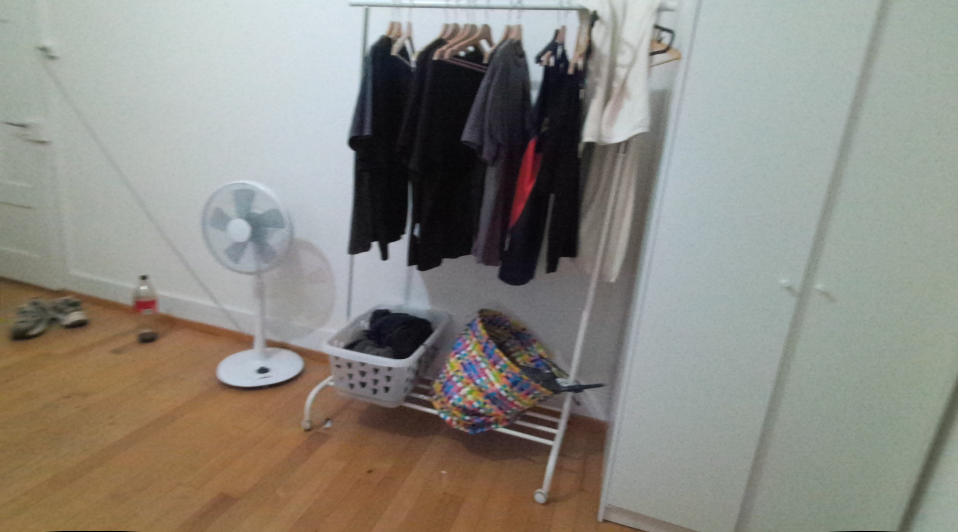
\includegraphics[width=\qwidth,trim={165.0000bp 10.0000bp 343.0000bp 72.0000bp},clip]{figures/results_native/qual/1_real_05320/0_image.png} &
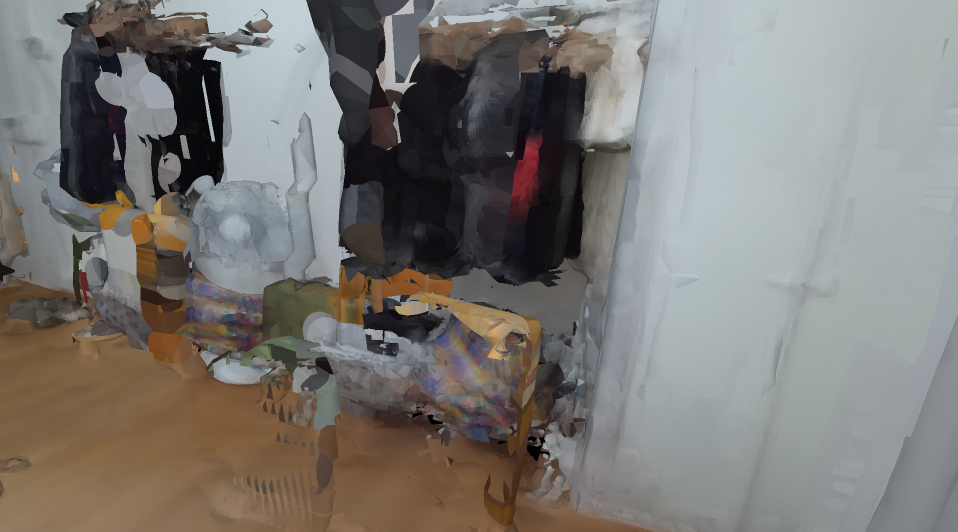
\includegraphics[width=\qwidth,trim={165.0000bp 10.0000bp 343.0000bp 72.0000bp},clip]{figures/results_native/qual/1_real_05320/1_khronos.png} &
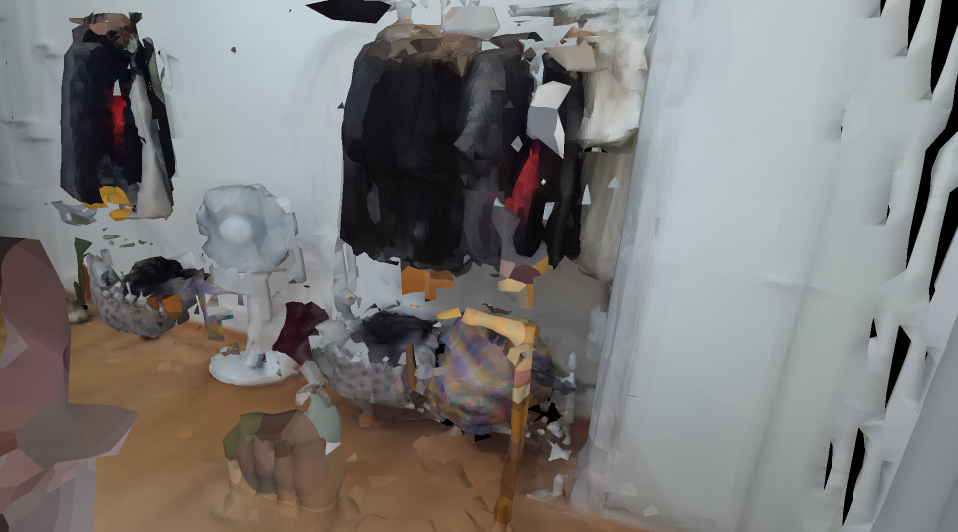
\includegraphics[width=\qwidth,trim={165.0000bp 10.0000bp 343.0000bp 72.0000bp},clip]{figures/results_native/qual/1_real_05320/2_panoptic.png} &
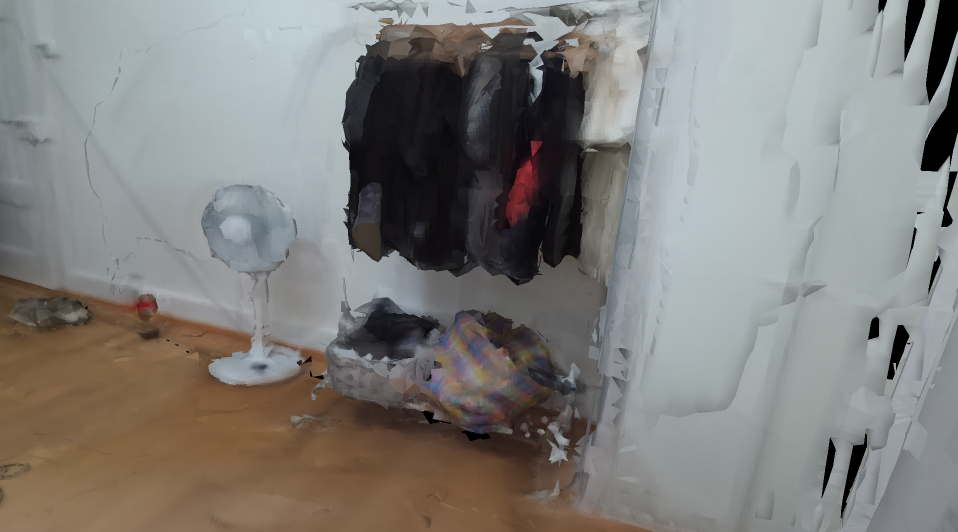
\includegraphics[width=\qwidth,trim={165.0000bp 10.0000bp 343.0000bp 72.0000bp},clip]{figures/results_native/qual/1_real_05320/3_ours_tsdf.png} &
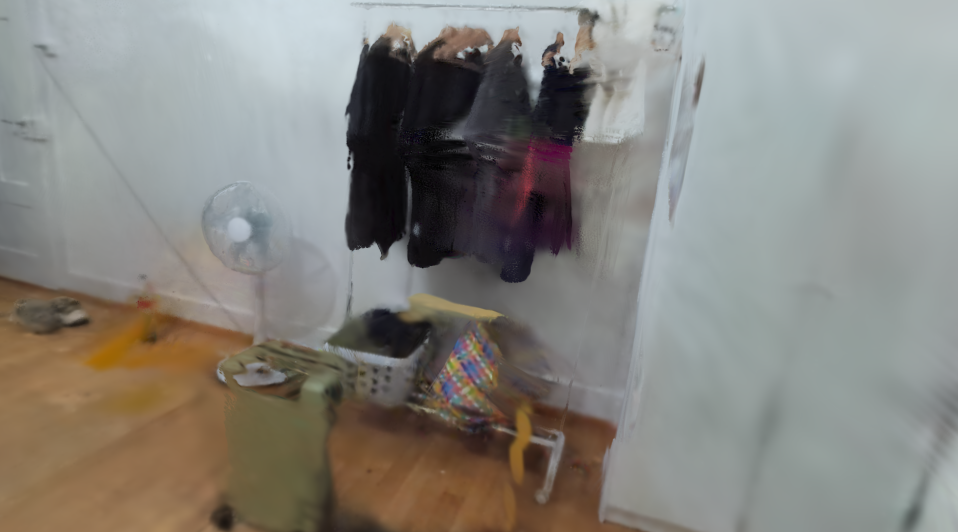
\includegraphics[width=\qwidth,trim={165.0000bp 10.0000bp 343.0000bp 72.0000bp},clip]{figures/results_native/qual/1_real_05320/4_game.png} &
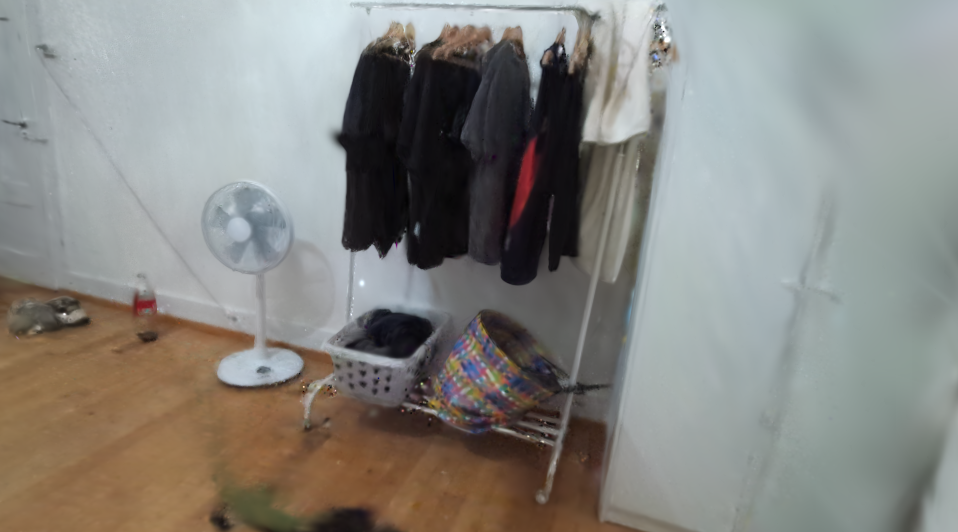
\includegraphics[width=\qwidth,trim={165.0000bp 10.0000bp 343.0000bp 72.0000bp},clip]{figures/results_native/qual/1_real_05320/5_ours_3dgs.png} &
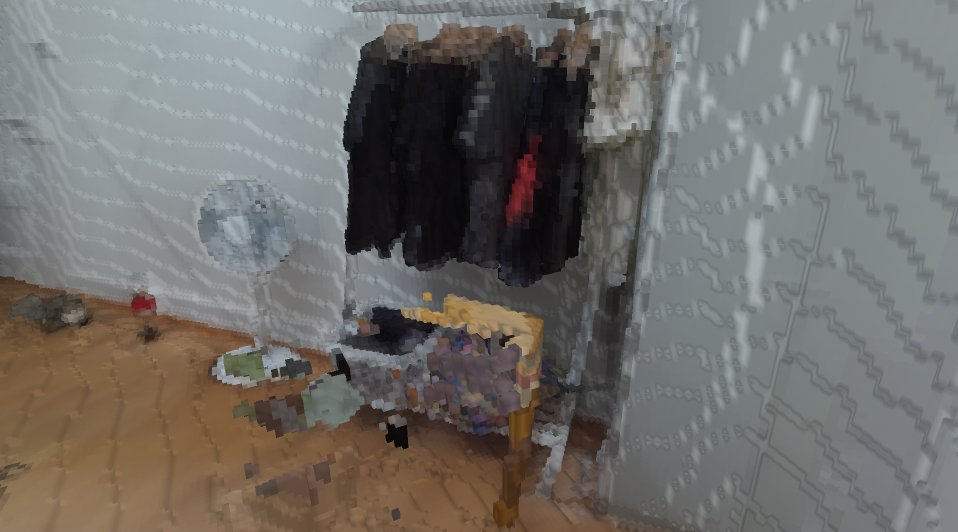
\includegraphics[width=\qwidth,trim={165.0000bp 10.0000bp 343.0000bp 72.0000bp},clip]{figures/results_native/qual/1_real_05320/6_wavemap.png} &
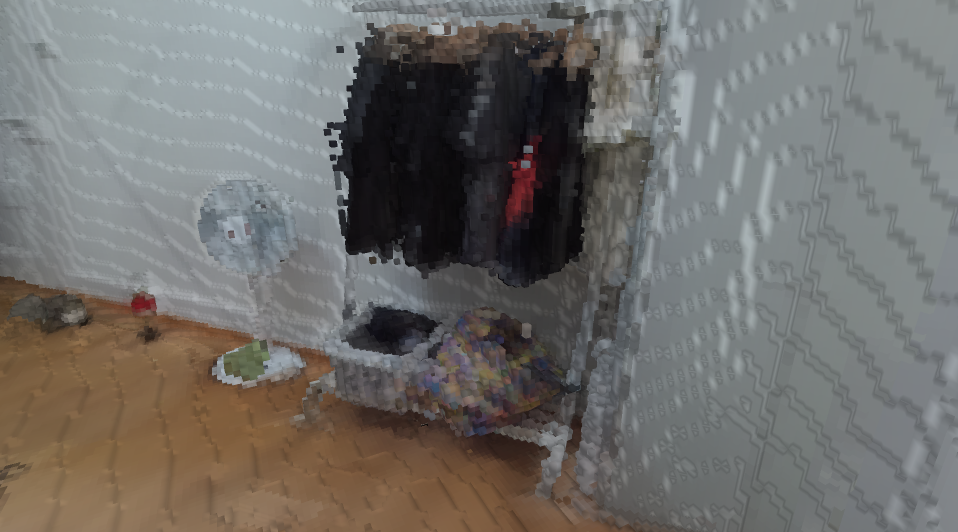
\includegraphics[width=\qwidth,trim={165.0000bp 10.0000bp 343.0000bp 72.0000bp},clip]{figures/results_native/qual/1_real_05320/7_ours_occ.png}\\[2pt]
% 2_real_02540 [105, 80, 550, 525]
\rotatebox{90}{BedRoom} &
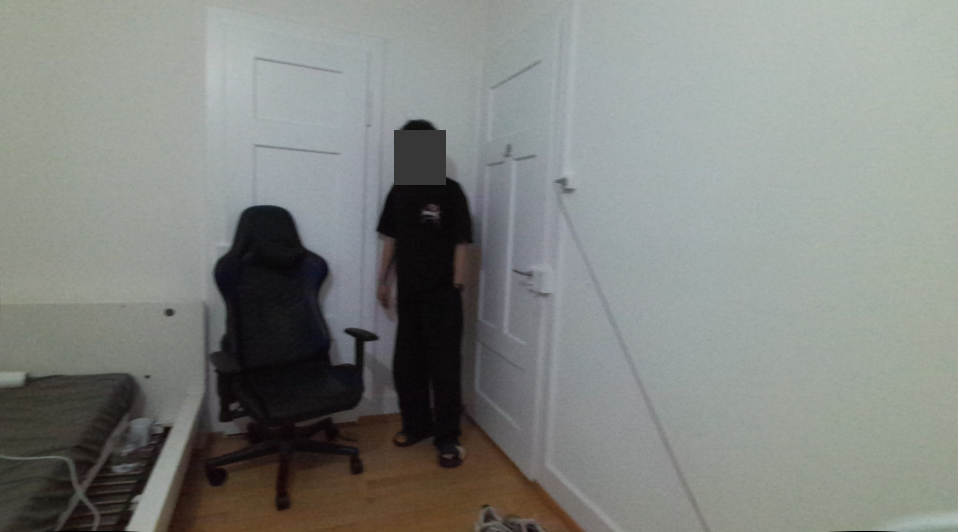
\includegraphics[width=\qwidth,trim={105.0000bp 7.0000bp 408.0000bp 80.0000bp},clip]{figures/privacy/face_redacted_5.png} &
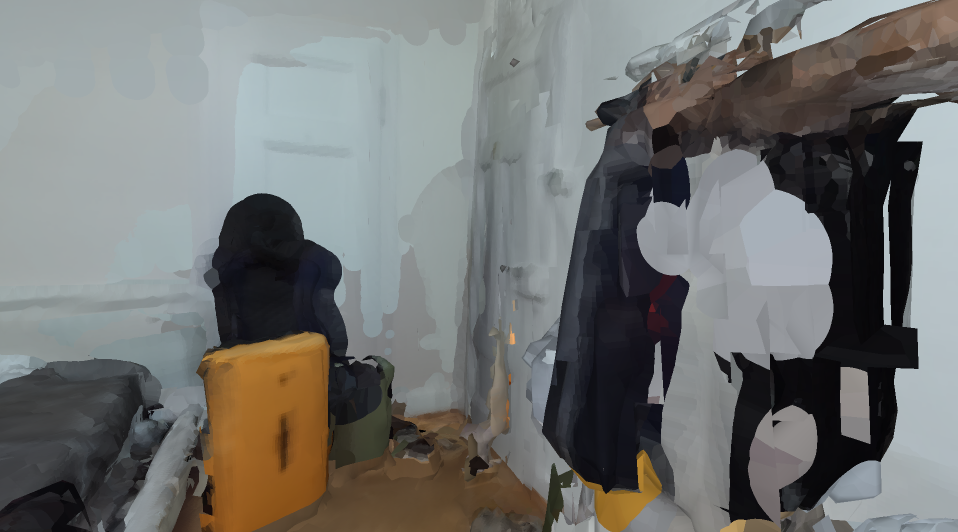
\includegraphics[width=\qwidth,trim={105.0000bp 7.0000bp 408.0000bp 80.0000bp},clip]{figures/results_native/qual/2_real_02540/1_khronos.png} &
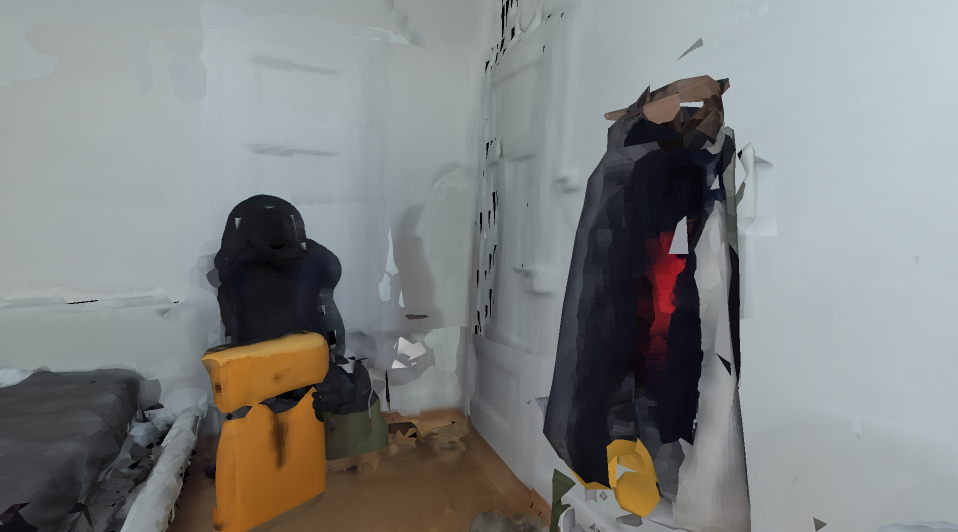
\includegraphics[width=\qwidth,trim={105.0000bp 7.0000bp 408.0000bp 80.0000bp},clip]{figures/results_native/qual/2_real_02540/2_panoptic.png} &
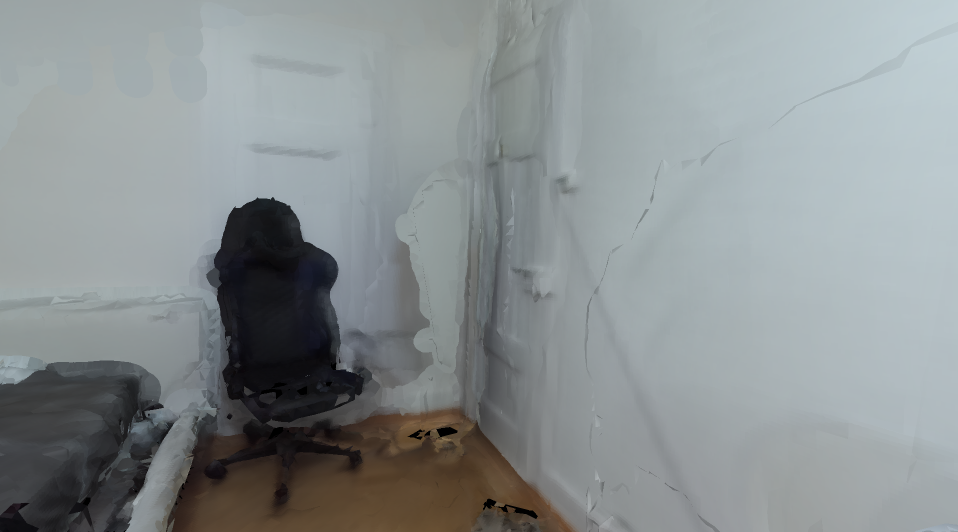
\includegraphics[width=\qwidth,trim={105.0000bp 7.0000bp 408.0000bp 80.0000bp},clip]{figures/results_native/qual/2_real_02540/3_ours_tsdf.png} &
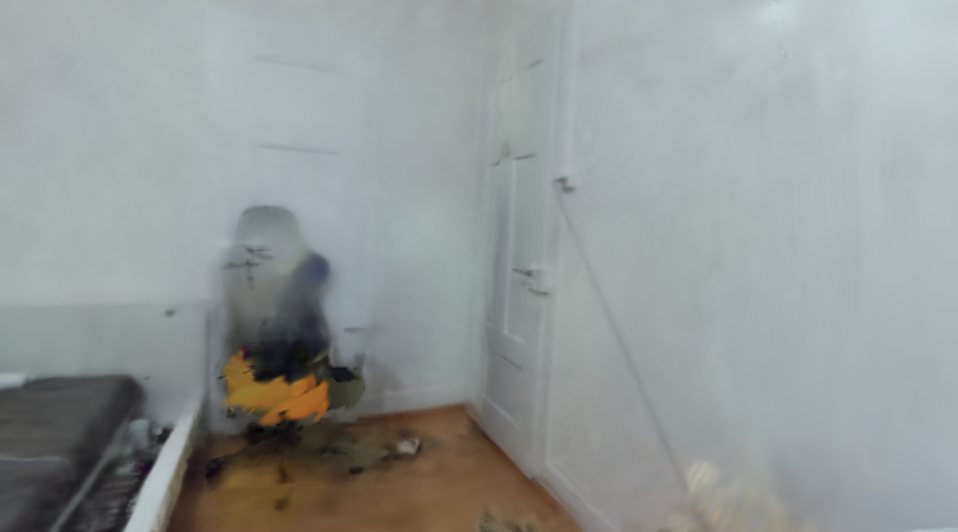
\includegraphics[width=\qwidth,trim={105.0000bp 7.0000bp 408.0000bp 80.0000bp},clip]{figures/results_native/qual/2_real_02540/4_game.png} &
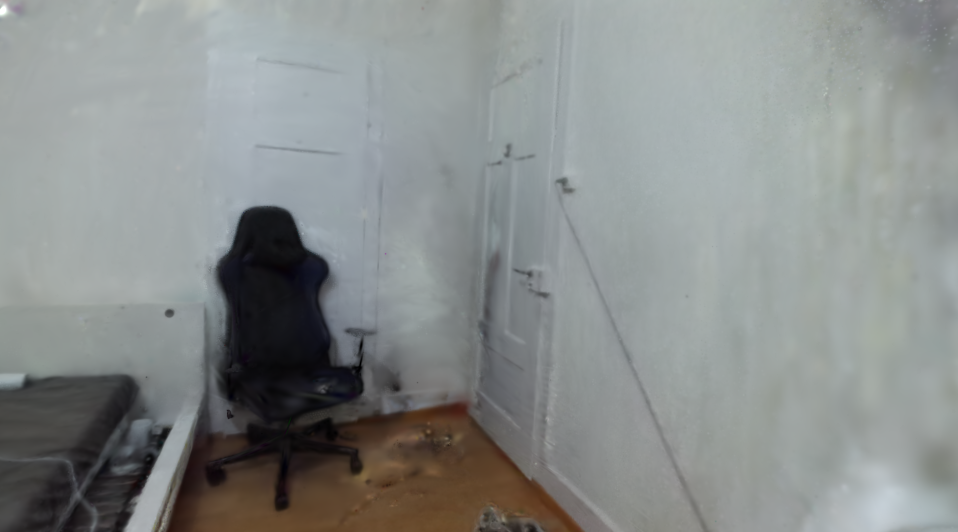
\includegraphics[width=\qwidth,trim={105.0000bp 7.0000bp 408.0000bp 80.0000bp},clip]{figures/results_native/qual/2_real_02540/5_ours_3dgs.png} &
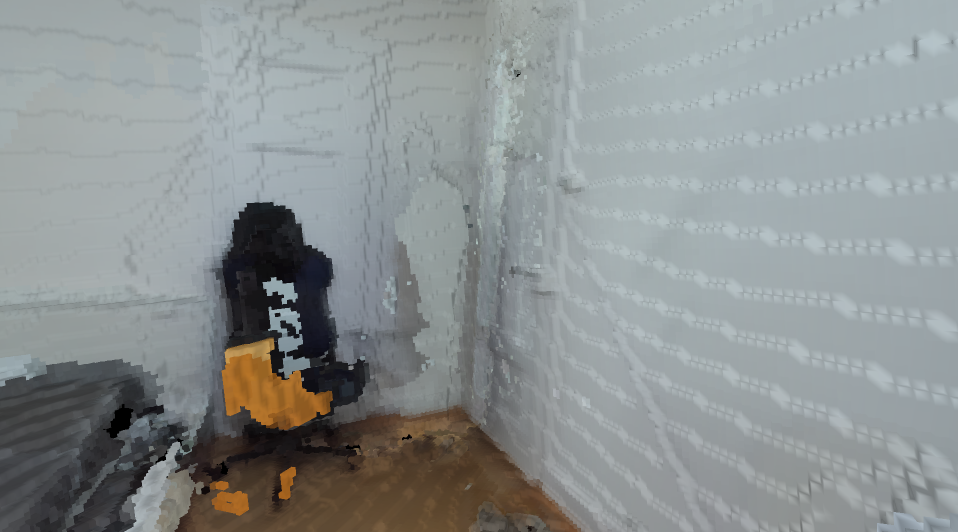
\includegraphics[width=\qwidth,trim={105.0000bp 7.0000bp 408.0000bp 80.0000bp},clip]{figures/results_native/qual/2_real_02540/6_wavemap.png} &
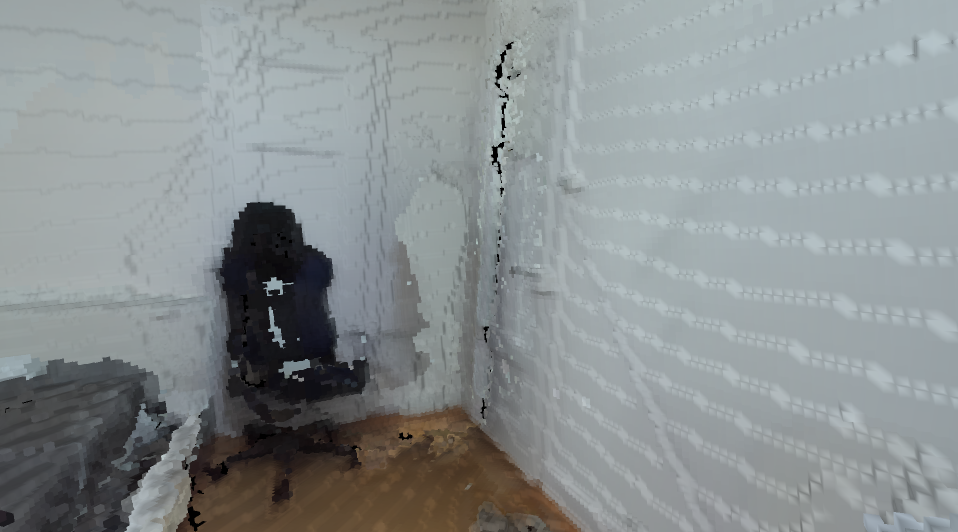
\includegraphics[width=\qwidth,trim={105.0000bp 7.0000bp 408.0000bp 80.0000bp},clip]{figures/results_native/qual/2_real_02540/7_ours_occ.png}\\[2pt]
% 3_sim_02850 [150, 15, 580, 445]
\rotatebox{90}{Home} &
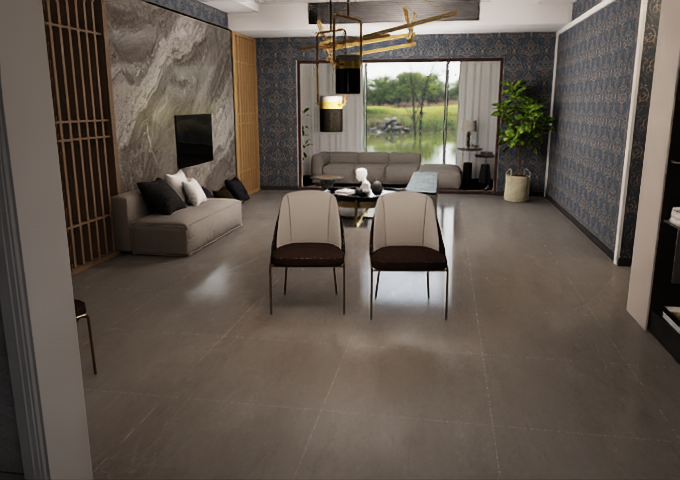
\includegraphics[width=\qwidth,trim={150.0000bp 35.0000bp 100.0000bp 15.0000bp},clip]{figures/results_native/qual/3_sim_02850/0_image.png} &
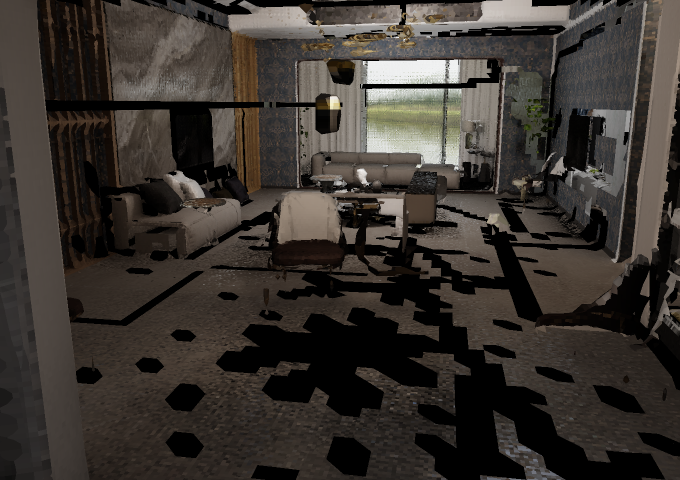
\includegraphics[width=\qwidth,trim={150.0000bp 35.0000bp 100.0000bp 15.0000bp},clip]{figures/results_native/qual/3_sim_02850/1_khronos.png} &
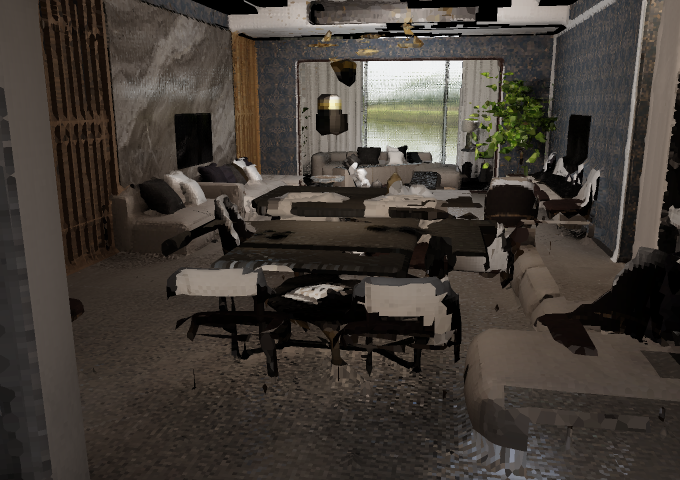
\includegraphics[width=\qwidth,trim={150.0000bp 35.0000bp 100.0000bp 15.0000bp},clip]{figures/results_native/qual/3_sim_02850/2_panoptic.png} &
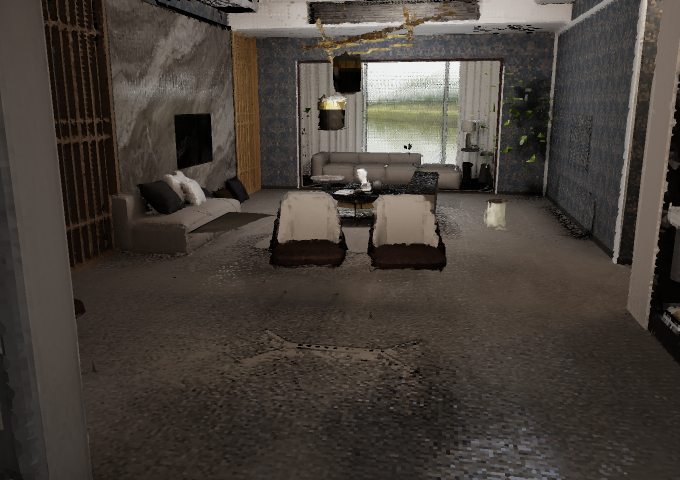
\includegraphics[width=\qwidth,trim={150.0000bp 35.0000bp 100.0000bp 15.0000bp},clip]{figures/results_native/qual/3_sim_02850/3_ours_tsdf.png} &
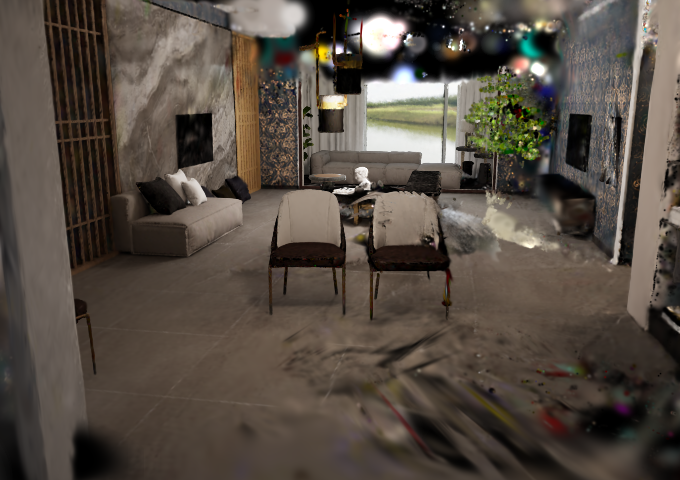
\includegraphics[width=\qwidth,trim={150.0000bp 35.0000bp 100.0000bp 15.0000bp},clip]{figures/results_native/qual/3_sim_02850/4_game.png} &
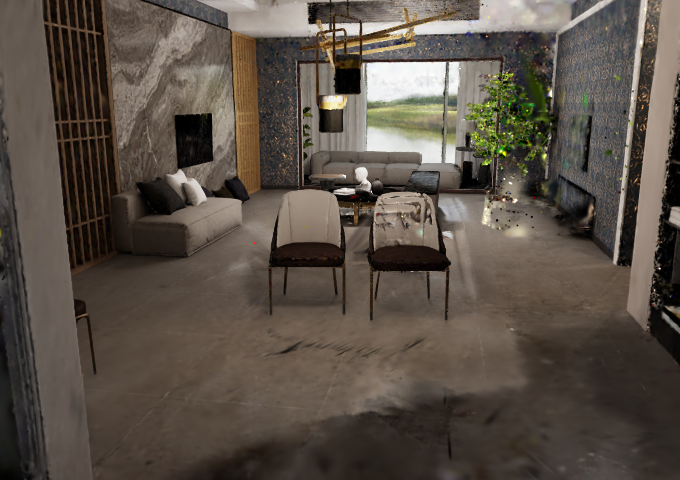
\includegraphics[width=\qwidth,trim={150.0000bp 35.0000bp 100.0000bp 15.0000bp},clip]{figures/results_native/qual/3_sim_02850/5_ours_3dgs.png} &
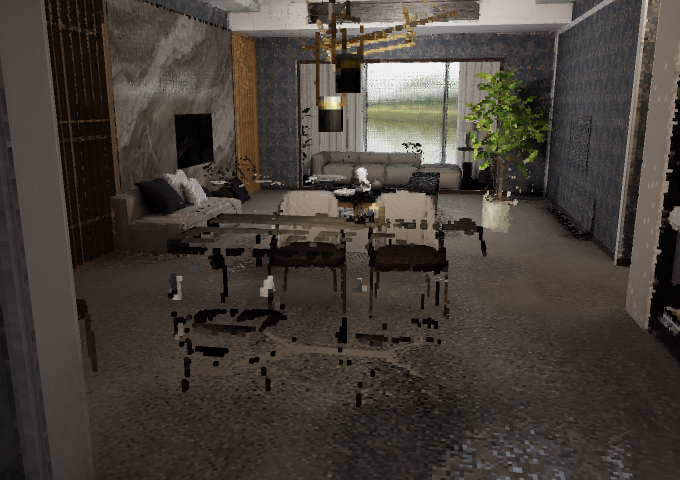
\includegraphics[width=\qwidth,trim={150.0000bp 35.0000bp 100.0000bp 15.0000bp},clip]{figures/results_native/qual/3_sim_02850/6_wavemap.png} &
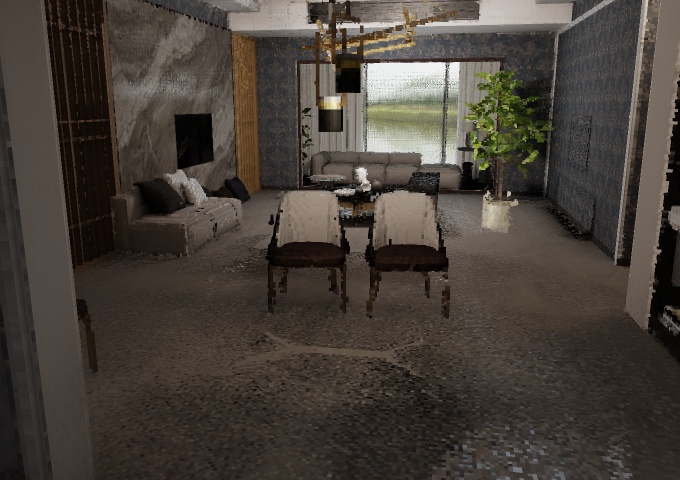
\includegraphics[width=\qwidth,trim={150.0000bp 35.0000bp 100.0000bp 15.0000bp},clip]{figures/results_native/qual/3_sim_02850/7_ours_occ.png}\\[2pt]
% 10_sim_03080 [100, 0, 580, 480]
\rotatebox{90}{Home} &
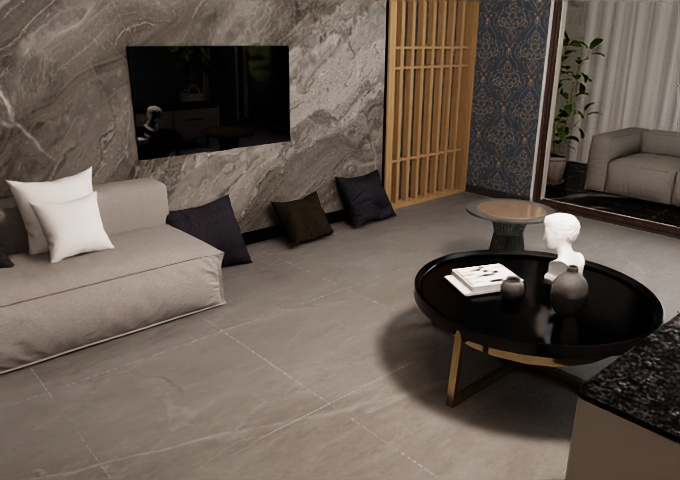
\includegraphics[width=\qwidth,trim={100bp 0bp 100bp 0bp},clip]{figures/results_native/qual/10_sim_03080/0_image.png} &
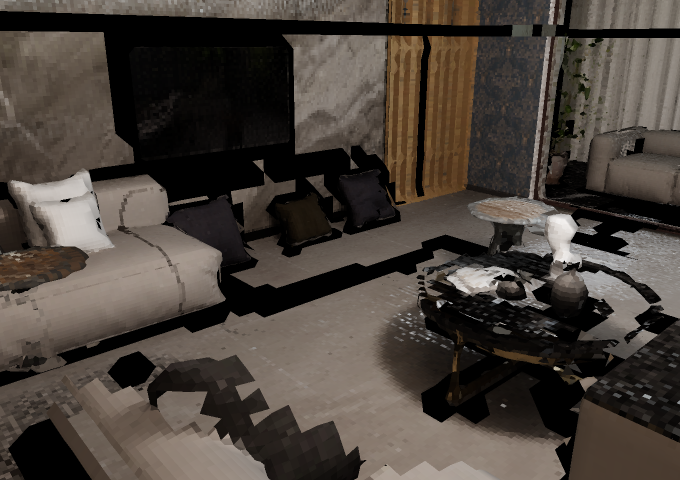
\includegraphics[width=\qwidth,trim={100bp 0bp 100bp 0bp},clip]{figures/results_native/qual/10_sim_03080/1_khronos.png} &
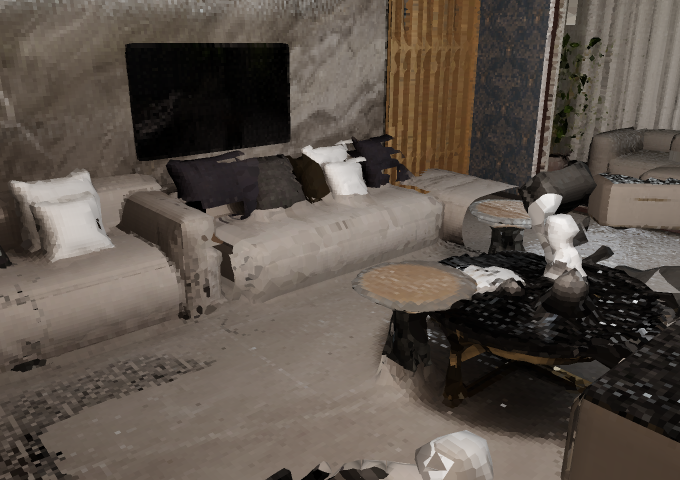
\includegraphics[width=\qwidth,trim={100bp 0bp 100bp 0bp},clip]{figures/results_native/qual/10_sim_03080/2_panoptic.png} &
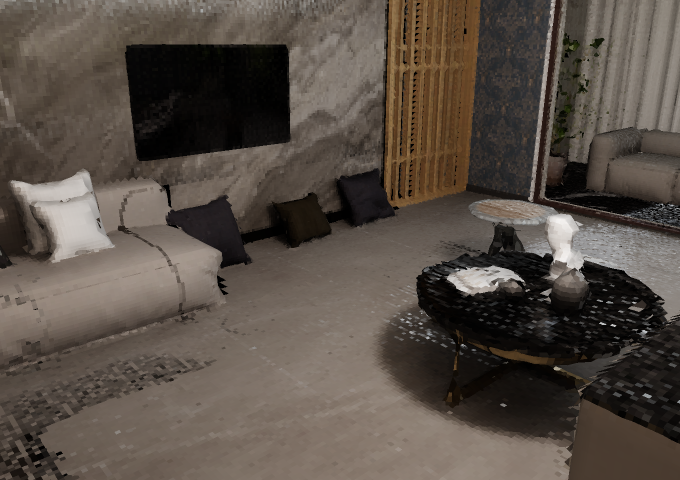
\includegraphics[width=\qwidth,trim={100bp 0bp 100bp 0bp},clip]{figures/results_native/qual/10_sim_03080/3_ours_tsdf.png} &
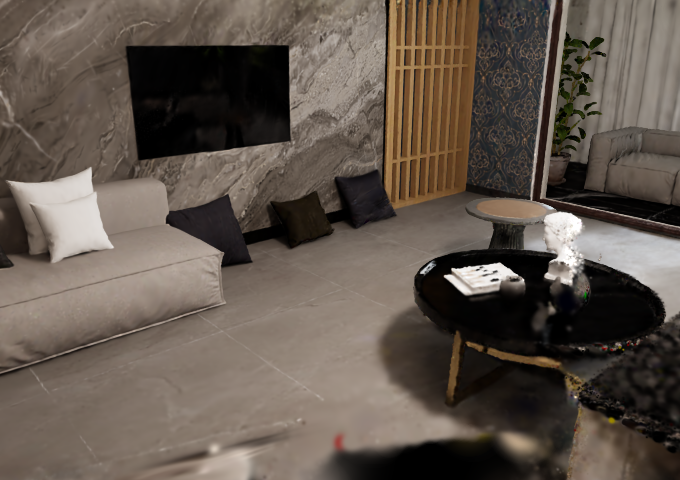
\includegraphics[width=\qwidth,trim={100bp 0bp 100bp 0bp},clip]{figures/results_native/qual/10_sim_03080/4_game.png} &
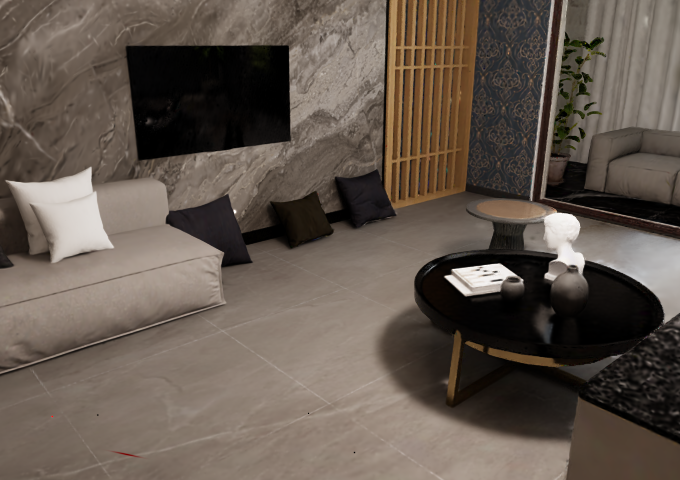
\includegraphics[width=\qwidth,trim={100bp 0bp 100bp 0bp},clip]{figures/results_native/qual/10_sim_03080/5_ours_3dgs.png} &
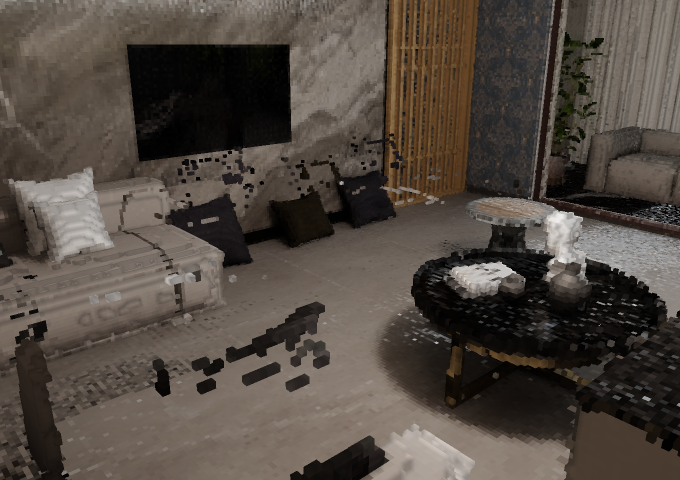
\includegraphics[width=\qwidth,trim={100bp 0bp 100bp 0bp},clip]{figures/results_native/qual/10_sim_03080/6_wavemap.png} &
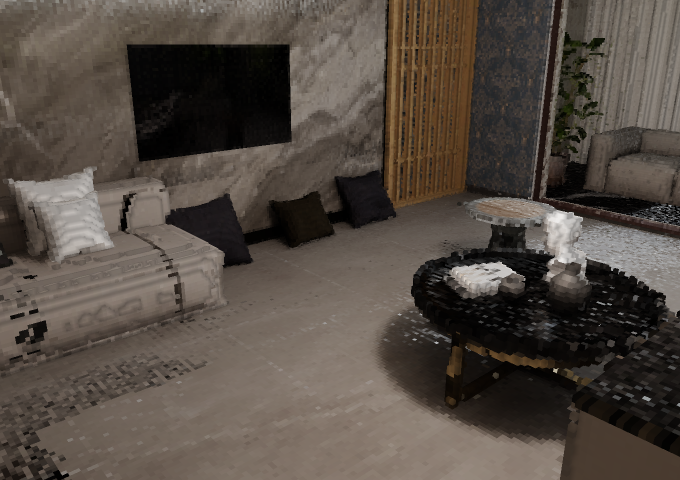
\includegraphics[width=\qwidth,trim={100bp 0bp 100bp 0bp},clip]{figures/results_native/qual/10_sim_03080/7_ours_occ.png}\\[2pt]
% 5_flat_00270 [160, 90, 550, 480]
\rotatebox{90}{Flat} &
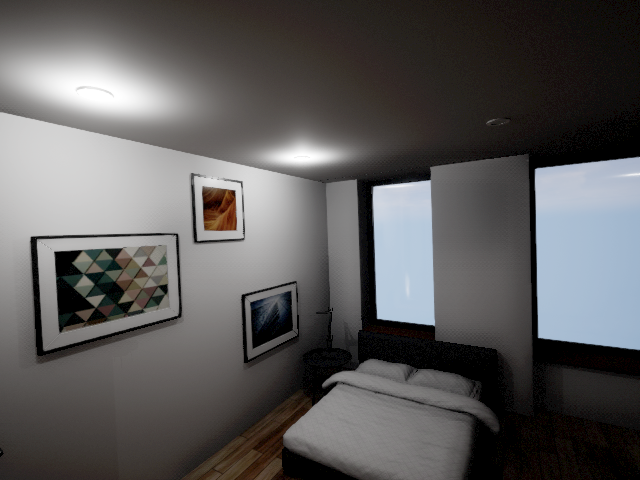
\includegraphics[width=\qwidth,trim={160.0000bp 0.0000bp 90.0000bp 90.0000bp},clip]{figures/results_native/qual/5_flat_00270/0_image.png} &
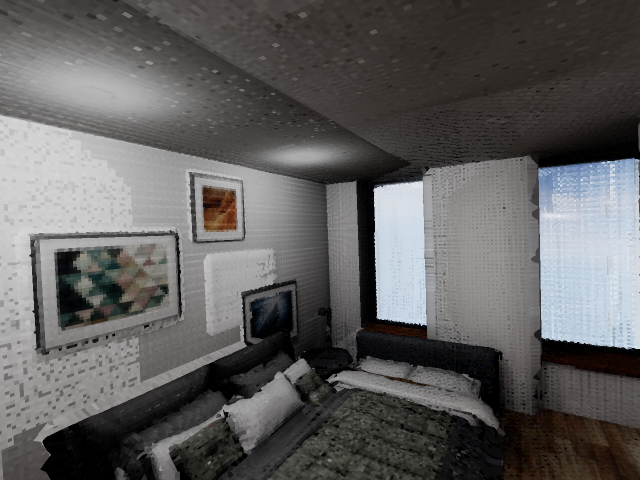
\includegraphics[width=\qwidth,trim={160.0000bp 0.0000bp 90.0000bp 90.0000bp},clip]{figures/results_native/qual/5_flat_00270/1_khronos.png} &
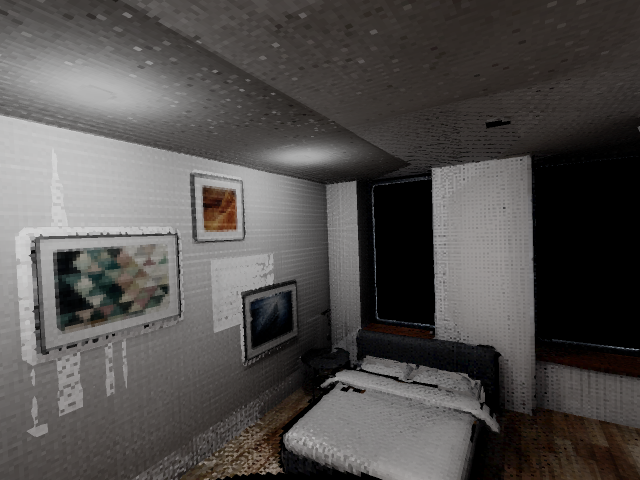
\includegraphics[width=\qwidth,trim={160.0000bp 0.0000bp 90.0000bp 90.0000bp},clip]{figures/results_native/qual/5_flat_00270/2_panoptic.png} &
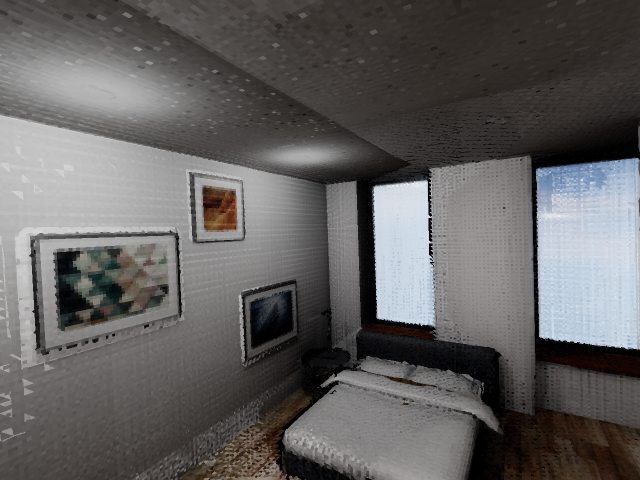
\includegraphics[width=\qwidth,trim={160.0000bp 0.0000bp 90.0000bp 90.0000bp},clip]{figures/results_native/qual/5_flat_00270/3_ours_tsdf.png} &
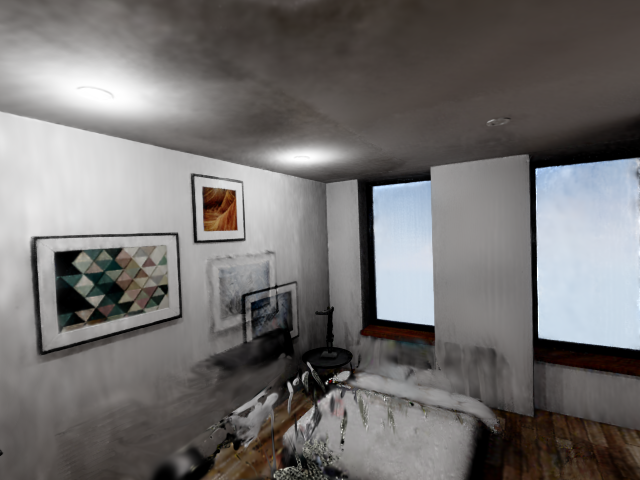
\includegraphics[width=\qwidth,trim={160.0000bp 0.0000bp 90.0000bp 90.0000bp},clip]{figures/results_native/qual/5_flat_00270/4_game.png} &
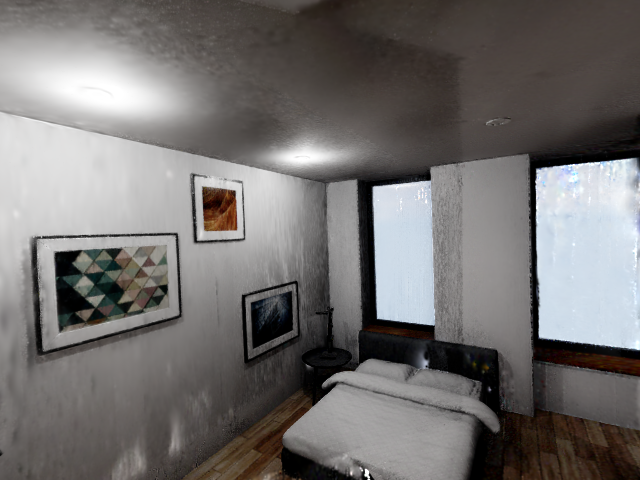
\includegraphics[width=\qwidth,trim={160.0000bp 0.0000bp 90.0000bp 90.0000bp},clip]{figures/results_native/qual/5_flat_00270/5_ours_3dgs.png} &
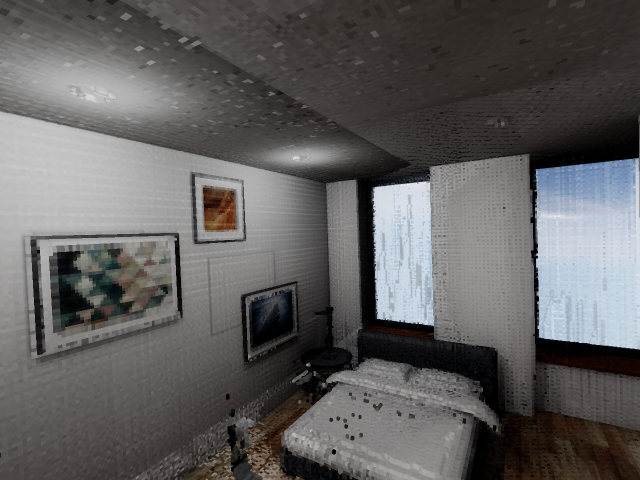
\includegraphics[width=\qwidth,trim={160.0000bp 0.0000bp 90.0000bp 90.0000bp},clip]{figures/results_native/qual/5_flat_00270/6_wavemap.png} &
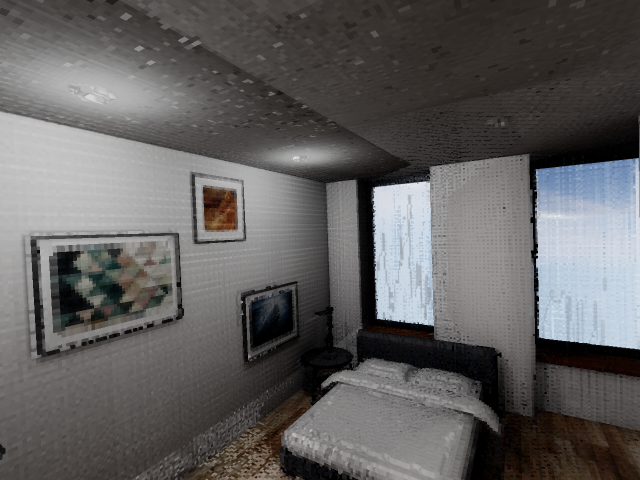
\includegraphics[width=\qwidth,trim={160.0000bp 0.0000bp 90.0000bp 90.0000bp},clip]{figures/results_native/qual/5_flat_00270/7_ours_occ.png}\\[2pt]
% 6_flat_00225 [100, 30, 525, 455]
\rotatebox{90}{Flat} &
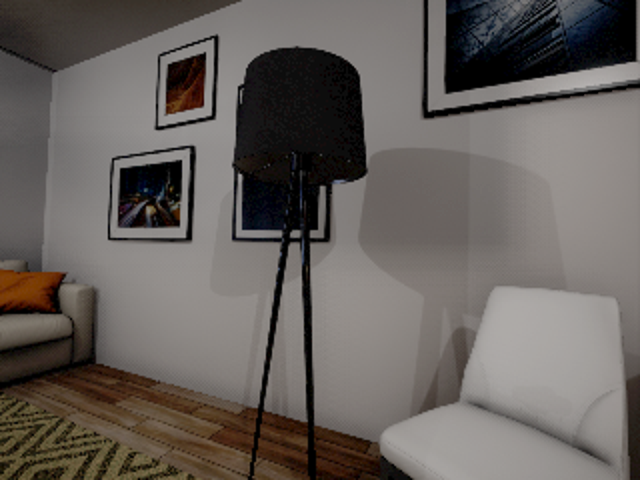
\includegraphics[width=\qwidth,trim={100.0000bp 25.0000bp 115.0000bp 30.0000bp},clip]{figures/results_native/qual/6_flat_00225/0_image.png} &
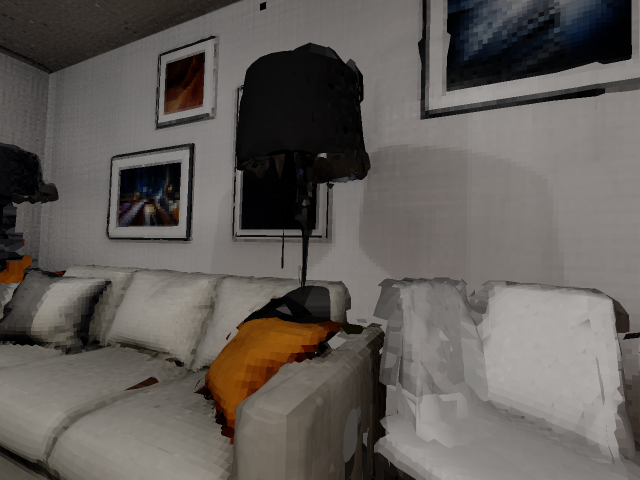
\includegraphics[width=\qwidth,trim={100.0000bp 25.0000bp 115.0000bp 30.0000bp},clip]{figures/results_native/qual/6_flat_00225/1_khronos.png} &
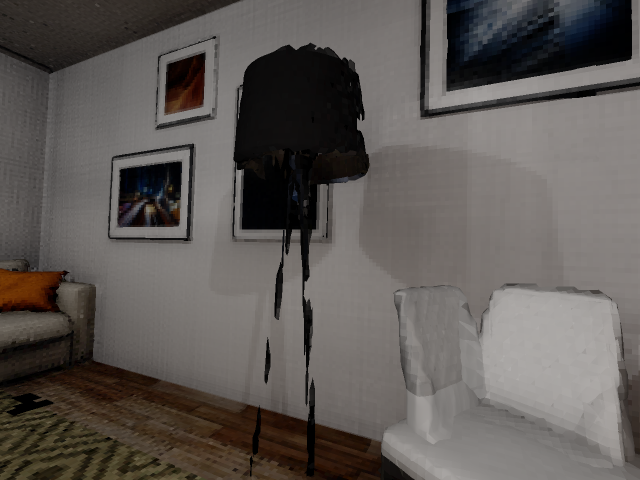
\includegraphics[width=\qwidth,trim={100.0000bp 25.0000bp 115.0000bp 30.0000bp},clip]{figures/results_native/qual/6_flat_00225/2_panoptic.png} &
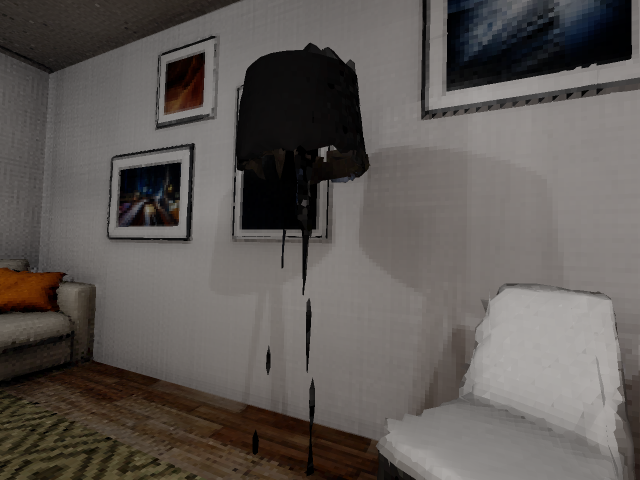
\includegraphics[width=\qwidth,trim={100.0000bp 25.0000bp 115.0000bp 30.0000bp},clip]{figures/results_native/qual/6_flat_00225/3_ours_tsdf.png} &
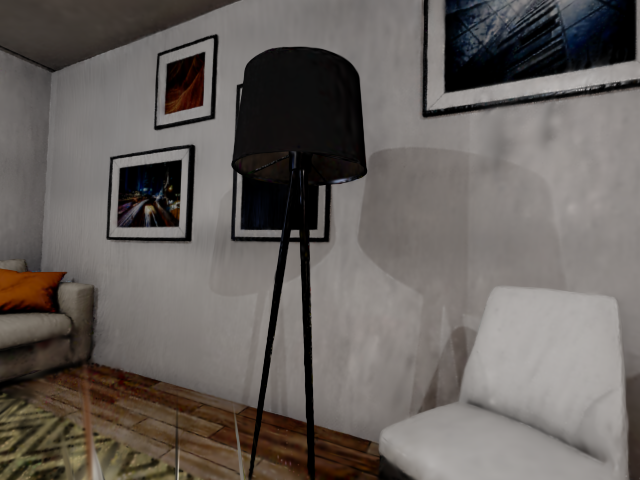
\includegraphics[width=\qwidth,trim={100.0000bp 25.0000bp 115.0000bp 30.0000bp},clip]{figures/results_native/qual/6_flat_00225/4_game.png} &
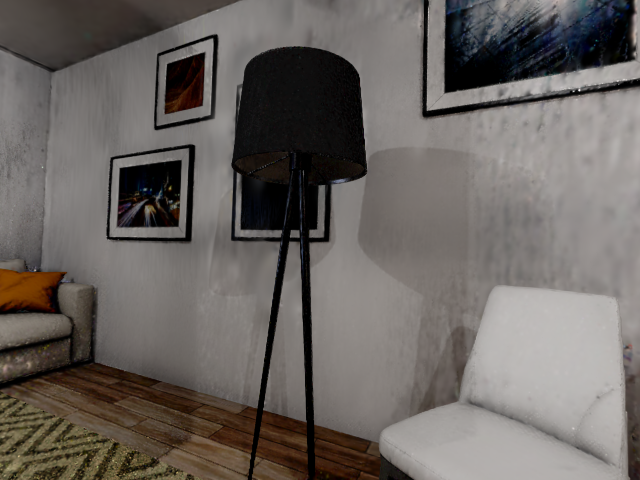
\includegraphics[width=\qwidth,trim={100.0000bp 25.0000bp 115.0000bp 30.0000bp},clip]{figures/results_native/qual/6_flat_00225/5_ours_3dgs.png} &
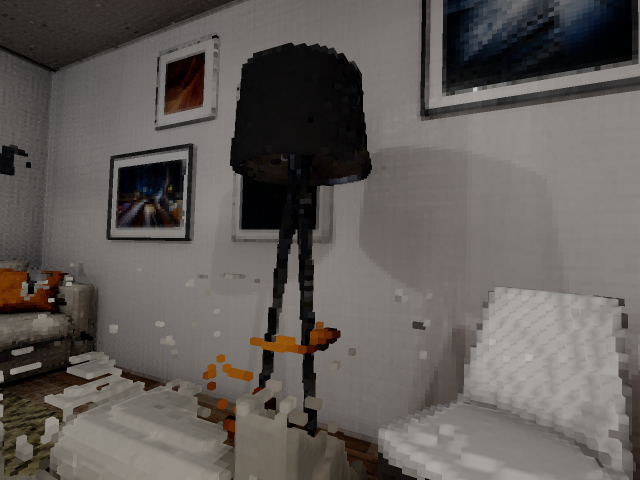
\includegraphics[width=\qwidth,trim={100.0000bp 25.0000bp 115.0000bp 30.0000bp},clip]{figures/results_native/qual/6_flat_00225/6_wavemap.png} &
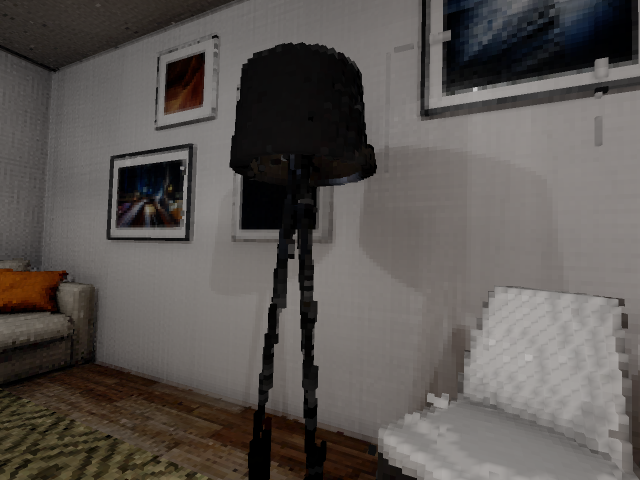
\includegraphics[width=\qwidth,trim={100.0000bp 25.0000bp 115.0000bp 30.0000bp},clip]{figures/results_native/qual/6_flat_00225/7_ours_occ.png}\\[2pt]
\end{tabular}\endgroup
\caption{\textbf{Scene updates across three representations.} Six views from the real room, synthetic apartment,
and Flat, with each method rendered at the image pose. Each row uses the same square crop and scale across methods.
TSDF and occupancy use reference colors. BedRoom occupancy panels use the capture-time maps; other panels
use final maps. Occupancy is visualized at 2\,cm resolution.}
\label{fig:qualitative}
\end{figure}

\FloatBarrier
{\small
\bibliographystyle{ieeenat_fullname}
\bibliography{main}
}
\end{document}
